\block{Descripción}{

	Los datos utilizados en este estudio provienen de diversos fuentes. Para la variable de producción se utilizo
	producción de energy provista por LUMA Energy como proxy del PIB \cite{BOROZAN2013373}. Mano de obra proviene del QCEW por el departamento del trabajo.
	Esto abarca a los 78 municipios en un periodo de 36 meses para un total de 2808 observaciones.

	\vspace{0.5em}

	Debido a la ausencia de datos directos de inversión de capital a nivel municipal, se desarrolló un modelo de \textbf{Capital Sintético} basado en la
	relación entre las importaciones nacionales, el empleo sectorial y la estacionalidad. Estos provisto por instituto de estadísticas de Puerto Rico

	\vspace{0.5em}
	Utilizamos un modelo jerárquico bayesiano para estimar el logaritmo de las importaciones ($I$) por sector ($s$) y tiempo ($t$):
	\begin{equation}
		\log(I_{s,t+1}) = \text{WALK}_{s,t} + \gamma \log(E_{s,t+1}) + \text{S}_{s,t} + \epsilon
	\end{equation}
	Donde:
	\begin{itemize}[leftmargin=1.5em]
		\item \textbf{Camino Aleatorio No Centrado:} Captura la evolución estructural del flujo de bienes de capital por sector, permitiendo derivas (\textit{drifts}) específicas.
		\item \textbf{Componente de Empleo ($\gamma$):} Vincula la intensidad laboral ($E$) con la necesidad de insumos importados. Se asume un prior \texttt{HalfNormal} para asegurar una relación positiva.
		\item \textbf{Estacionalidad de Fourier ($S_{s,t}$):} Captura ciclos anuales de importación mediante términos de seno y coseno ($\sin, \cos$).
	\end{itemize}

	\begin{tikzfigure}[Estimacion de importaciones del sector 11]
		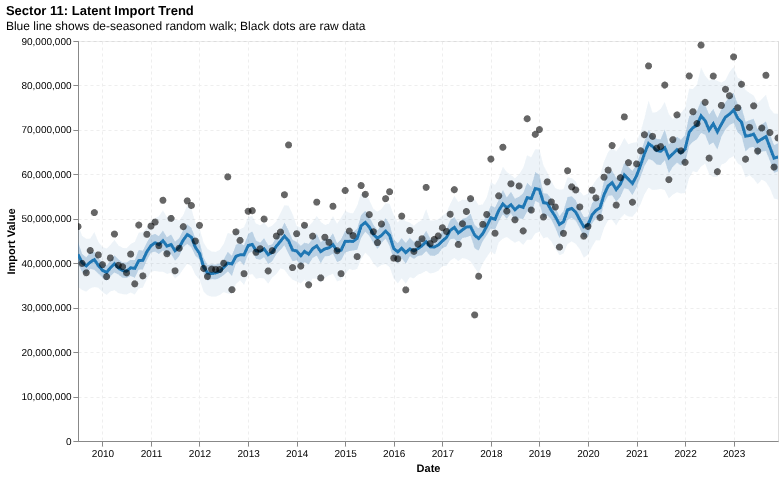
\includegraphics[width=1\linewidth]{assets/visualization.png}
	\end{tikzfigure}

	\begin{center}
		\begin{tabular}{l c c c}
			\hline
			\textbf{Estadístico} & \textbf{Capital ($K$)} & \textbf{Trabajo ($L$)} & \textbf{Energía ($E$)} \\
			\hline
			Promedio (Media)     & $3.50 \times 10^9$     & 14956.25               & $1.73 \times 10^7$     \\
			Desv. Estándar       & $1.05 \times 10^9$     & 47974.77               & $3.04 \times 10^7$     \\
			Mínimo               & $6.03 \times 10^7$     & 330.00                 & $-1.54 \times 10^7$    \\
			\hline
			Percentil 25\%       & $3.47 \times 10^9$     & 2669.75                & $4.90 \times 10^6$     \\
			Mediana (50\%)       & $3.81 \times 10^9$     & 4499.00                & $8.63 \times 10^6$     \\
			Percentil 75\%       & $4.18 \times 10^9$     & 9527.25                & $1.74 \times 10^7$     \\
			Máximo               & $4.67 \times 10^9$     & 434890.00              & $2.88 \times 10^8$     \\
			\hline
		\end{tabular}
	\end{center}
	\vspace{1em}
	\small \textit{Nota: Capital y Energía se presentan en niveles sintéticos antes de la transformación logarítmica.}
}
